\documentclass[11pt]{article}
\usepackage[a4paper,margin=1.8cm]{geometry}
\usepackage{booktabs,tabularx,array,graphicx}
\usepackage[hidelinks]{hyperref}
\setlength{\emergencystretch}{3em}
\newcommand{\cges}{C\textsuperscript{2}GES}
\title{Supplementary Materials for\\
\cges{}: A Diagnostic Evaluation of Role-Conditioned Extractive Summarization for Long Power-System Technical Reports}
\author{Bijing Liu and Yong Yang}
\date{}
\begin{document}
\maketitle

\section*{Contents and Data Files}

This supplement separates scientific interpretation from implementation records. It contains twenty tables and two figures referenced by the main manuscript. The main-text evidence-layer table (``Evidence layers and claim bounds'') states the four evaluation layers and what each may and may not support; the tables below are implementation and exploratory-component records for those layers, not a confirmatory external test. Paths below are relative to the C2GES release root. Machine-readable files are provided under \nolinkurl{03_Reproducibility/Data/}: the non-verbatim sampling frames, aggregate metrics, paired ROUGE-L differences, output-length records, exact sign-flip results, page locators, component-factorial diagnostics, and development-only calibration report. Source PDFs and verbatim extracted passages are excluded because third-party redistribution permission has not been established.

\section*{Table S1. Rights-Safe Sampling Frame}

The complete 40-row sampling frame is supplied as \nolinkurl{03_Reproducibility/Data/rights_safe_metadata/rights_safe_report_metadata.csv}. Its 23 fields include the report identifier, source locator, split, series identifier, inclusion decision, source-file hash, and redistribution status; it contains no report passages.

\begin{center}
\begin{tabular}{lr}
\toprule
Quantity & Value\\
\midrule
Inspected complete PDFs & 40\\
Declared pages & 3200\\
Retained / excluded reports & 27 / 13\\
Development / test reports & 12 / 15\\
Non-summary candidates & 12,924\\
\bottomrule
\end{tabular}
\end{center}

\section*{Table S2. Output-Length Records}

The complete 14 condition--budget summary is supplied as \nolinkurl{03_Reproducibility/Data/postrun_diagnostics/output_length_summary.csv}; per-report values are in \nolinkurl{03_Reproducibility/Data/postrun_diagnostics/output_length_per_report.csv}. ``Unrenorm. removal'' denotes the unrenormalized coefficient-removal comparison.

\begin{center}
\small
\begin{tabular}{llrrrrr}
\toprule
$K$ & Condition & Mean words & Mean chars. & $>100$ & Table & Max. words\\
\midrule
5 & Full \cges{} & 287.7 & 1843.6 & 12 & 14 & 140\\
5 & Unrenorm. removal & 329.0 & 2099.9 & 15 & 16 & 270\\
5 & Semantic-MMR & 184.7 & 1242.1 & 5 & 9 & 138\\
5 & TextRank & 177.0 & 1125.1 & 1 & 7 & 124\\
10 & Full \cges{} & 568.9 & 3619.5 & 25 & 26 & 270\\
10 & Unrenorm. removal & 596.9 & 3822.5 & 28 & 26 & 270\\
10 & Semantic-MMR & 354.5 & 2361.2 & 7 & 16 & 138\\
10 & TextRank & 369.0 & 2329.7 & 4 & 18 & 130\\
\bottomrule
\end{tabular}
\end{center}

\section*{Table S3. Corpus and Implementation Checks}

\begin{center}
\begin{tabularx}{\textwidth}{Xr}
\toprule
Checked property & Recorded result\\
\midrule
Reference/body page-interval overlap & 0\\
Normalized exact candidate/reference matches & 0\\
Normalized common substrings of at least 50 characters & 0\\
Report--condition--budget records / expected records & 210 / 210\\
Selected source references resolved to a valid page & 1575 / 1575\\
Maximum path expansions / configured limit & 19,638 / 2,000,000\\
Maximum qualifying paths / configured limit & 16,182 / 250,000\\
Full/unrenormalized-removal score comparisons changed & 9774 / 19,008\\
Report--budget selection sequences changed & 28 / 30\\
Aggregate and paired-contrast recomputation & Exact agreement\\
\bottomrule
\end{tabularx}
\end{center}

\begin{sloppypar}
Aggregate values are available at \nolinkurl{03_Reproducibility/Data/audits/aggregate_metrics.json}; non-verbatim paired differences and page locators are available at \nolinkurl{03_Reproducibility/Data/figure_inputs/paired_rougel_differences_nonverbatim.csv} and \nolinkurl{03_Reproducibility/Data/postrun_diagnostics/selected_page_locator.csv}. Detailed checks are retained with the corresponding code and archived run records. Passing these checks establishes consistency of the reported computation; it does not determine semantic summary quality.
\end{sloppypar}

\section*{Table S4. Exact Paired Sign-Flip Sensitivity}

For each contrast, all $2^{15}=32{,}768$ report-level sign assignments were enumerated. The procedure assumes report-level independence and sign exchangeability. Holm adjustment treats the six values as one family.

\begin{center}
\small
\begin{tabular}{llrrr}
\toprule
$K$ & Baseline & Signs $+/-/0$ & Exact $p$ & Holm-adjusted $p$\\
\midrule
5 & Unrenorm. removal & 7/7/1 & 0.436768 & 0.436768\\
5 & Semantic-MMR & 14/1/0 & 0.000305 & 0.001526\\
5 & TextRank & 14/1/0 & 0.000122 & 0.000732\\
10 & Unrenorm. removal & 6/8/1 & 0.200684 & 0.401367\\
10 & Semantic-MMR & 11/4/0 & 0.006592 & 0.026367\\
10 & TextRank & 13/2/0 & 0.009644 & 0.028931\\
\bottomrule
\end{tabular}
\end{center}

These post-result values are sensitivity analyses. The main manuscript emphasizes effect sizes, paired distributions, and report-composition intervals.

The complete machine-readable result is \nolinkurl{03_Reproducibility/Data/postrun_sensitivity/exact_signflip_results.csv}; the JSON file in the same directory retains the report-level non-verbatim deltas used in the calculation.

\section*{Table S5. Post-Access External-Series Inventory}

The fixed exploratory inventory contained eight public power-system reports from four organizations. Seven PDFs were acquired and analyzed; the NESO item returned HTTP 403 and was retained as a documented acquisition failure rather than replaced. Metadata or search snippets had been seen before the protocol was frozen, so all rows are classified as exploratory and none permits a confirmatory claim.

\begin{center}
\small
\begin{tabular}{lrrl}
\toprule
Organization & Fixed & Analyzed & Evidence status\\
\midrule
ENTSO-E & 3 & 3 & Post-access exploratory\\
NERC & 3 & 3 & Post-access exploratory\\
NESO & 1 & 0 & Acquisition failed (HTTP 403)\\
Transpower & 1 & 1 & Post-access exploratory\\
\midrule
Total & 8 & 7 & Confirmatory claims disallowed\\
\bottomrule
\end{tabular}
\end{center}

The non-verbatim record, source pages, direct-download locators, access date, and redistribution status are supplied in \nolinkurl{03_Reproducibility/Data/exploratory_external_v0/EXPLORATORY_EXTERNAL_INVENTORY.csv}.

\section*{Table S6. Controlled Comparator and Budget Conditions}

\begin{center}
\small
\begin{tabularx}{\textwidth}{lXX}
\toprule
Control & Frozen implementation & Diagnostic purpose\\
\midrule
Candidate pool & One layout-filtered pool per report for every method & Removes candidate-access asymmetry\\
Output budget & Complete-ranking greedy selection at 110 and 260 words; no sentence truncation & Matches emitted information quantity\\
Development opportunity & Nine configurations for each tunable system in the exploratory registry & Balances search opportunity\\
Series unit & Seven reports in seven distinct series & Supports equal-series contrasts and LOSO checks\\
Component scale & Positive weights renormalized to sum to one & Separates component removal from score-scale change\\
Failure policy & Every fixed item retained; execution status saved per cell & Prevents silent replacement or deletion\\
\bottomrule
\end{tabularx}
\end{center}

The v3 run completed all 182 condition--report--budget cells. These controls were fixed after source access and therefore improve internal comparability without converting the pilot into a prospective confirmatory experiment.

\section*{Table S7. Principal Component Contrasts}

\begin{center}
\small
\resizebox{\textwidth}{!}{%
\begin{tabular}{llrrrr}
\toprule
Family & Contrast and budget & Mean $\Delta$ R-L & 95\% cluster interval & Exact $p$ & Holm $p$\\
\midrule
Incremental & AB-5 $-$ AB-6, 110 & -0.00799 & [-0.01949, 0.00149] & 0.34375 & 1.00000\\
Incremental & AB-5 $-$ AB-6, 260 & -0.00718 & [-0.01855, 0.00151] & 0.28125 & 1.00000\\
Graph type & G-T $-$ G-U, 110 &  0.00139 & [-0.01481, 0.01959] & 0.90625 & 0.90625\\
Graph type & G-T $-$ G-U, 260 & -0.00544 & [-0.01640, 0.00594] & 0.35938 & 0.71875\\
Factorial & Reservation main, 110 & -0.00971 & [-0.01751, -0.00244] & 0.04688 & 0.23438\\
Factorial & Path main, 110 & -0.00247 & [-0.01787, 0.01333] & 0.79688 & 1.00000\\
Factorial & Interaction, 110 & -0.01104 & [-0.03173, 0.00264] & 0.34375 & 1.00000\\
Factorial & Reservation main, 260 &  0.00047 & [-0.00387, 0.00530] & 0.87500 & 1.00000\\
Factorial & Path main, 260 & -0.01034 & [-0.01871, -0.00371] & 0.03125 & 0.18750\\
Factorial & Interaction, 260 &  0.00632 & [-0.00222, 0.01602] & 0.25000 & 1.00000\\
\bottomrule
\end{tabular}}
\end{center}

No component contrast survived its separately defined Holm family. Intervals use series-cluster resampling, and exact values enumerate the $2^7$ series sign assignments. Full series effects, standardized paired effects, and leave-one-series-out estimates are provided in \nolinkurl{factorial_series_effects.csv} and \nolinkurl{factorial_loso.csv} under the v3 factorial directory.

\section*{Table S8. Complete AB-0--AB-6 Component Chain}

\begin{center}
\scriptsize
\resizebox{\textwidth}{!}{%
\begin{tabular}{lrrrrrrr}
\toprule
Budget & Condition & R-L & Redundancy & Role cov. & Edge cov. & Words/util. & Time (s)/MB\\
\midrule
110 & AB-0 & 0.1564 & 0.2308 & 0.286 & 0.662 & 108.4/0.986 & 0.269/1.04\\
110 & AB-1 & 0.1582 & 0.1527 & 0.524 & 0.869 & 108.4/0.986 & 0.268/1.04\\
110 & AB-2 & 0.1696 & 0.0783 & 1.000 & 0.890 & 108.1/0.983 & 0.253/1.03\\
110 & AB-3 & 0.1707 & 0.0800 & 1.000 & 0.971 & 108.1/0.983 & 0.248/1.03\\
110 & AB-4 & 0.1577 & 0.0564 & 1.000 & 0.964 & 109.0/0.991 & 0.249/1.03\\
110 & AB-5 & 0.1588 & 0.0508 & 1.000 & 0.964 & 108.6/0.987 & 0.252/1.06\\
110 & AB-6 & 0.1668 & 0.0595 & 1.000 & 0.948 & 108.4/0.986 & 0.252/1.08\\
\midrule
260 & AB-0 & 0.1687 & 0.1799 & 0.429 & 0.626 & 258.0/0.992 & 0.350/1.12\\
260 & AB-1 & 0.1873 & 0.1185 & 0.714 & 0.885 & 259.3/0.997 & 0.347/1.12\\
260 & AB-2 & 0.1843 & 0.1128 & 1.000 & 0.906 & 258.6/0.995 & 0.305/1.12\\
260 & AB-3 & 0.1848 & 0.1038 & 1.000 & 0.971 & 257.7/0.991 & 0.314/1.12\\
260 & AB-4 & 0.1805 & 0.0915 & 1.000 & 1.000 & 257.9/0.992 & 0.313/1.12\\
260 & AB-5 & 0.1772 & 0.0509 & 1.000 & 1.000 & 258.1/0.993 & 0.344/1.45\\
260 & AB-6 & 0.1844 & 0.0747 & 1.000 & 0.984 & 257.4/0.990 & 0.342/1.46\\
\bottomrule
\end{tabular}}
\end{center}

All failure rates were zero. Runtime is the recorded per-report estimate and memory is Python peak allocation; the separately loaded embedding model is excluded. Role and edge coverage measure heuristic formal coverage, not human-validated semantic correctness.

\section*{Table S9. Adjacent-Corpus Construct Audit of Role and Edge Cues}

Two public corpora carrying human annotation were used to bound what the lexical role and edge channels can carry. The deterministic role rule and its transition rule were applied unchanged; neither corpus is redistributed, and both must be obtained from their original distributors. This is an adjacent-corpus construct audit, not the domain expert adjudication reserved in the main text.

\begin{center}
\small
\resizebox{\textwidth}{!}{%
\begin{tabular}{llrrrrl}
\toprule
Corpus & Endpoint & Units & Human positive rate & Precision & Recall & Note\\
\midrule
GUM eRST & Dominant role assigned & 7678 EDUs & --- & --- & --- & 349 units (4.55\%)\\
GUM eRST & Admissible typed edge & 7285 pairs & 0.179 & not estimable & not estimable & 45 pairs (0.62\%) had role evidence on both units\\
EBM-NLP & interventions $\rightarrow$ mitigation & 2139 sentences & 0.524 & 0.610 & 0.064 & 382 sentences (17.9\%) received a dominant role\\
EBM-NLP & outcomes $\rightarrow$ impact & 2139 sentences & 0.519 & 0.807 & 0.060 & same sentence set as above\\
\bottomrule
\end{tabular}}
\end{center}

The GUM rows use the human enhanced-RST relation labels of the Georgetown University Multilayer corpus; the EBM-NLP rows use test spans annotated by medical professionals, with two roles mapped onto C2GES role names (intervention to mitigation, outcome to impact) and the participant label reported as unmapped. The cues are precise when they fire and sparse and genre-bound in general text; neither row closes any precondition of the annotated-study gate in the main text, and no row supports a role, edge, path, faithfulness, or omission claim.

\section*{Table S10. External Prospective Evaluation on a New Report Family}

The inventory, reference rule, budgets, comparators, endpoints and statistics were frozen before any score was computed (protocol and amendments in \nolinkurl{03_Reproducibility/Data/external_prospective_v1/}). The corpus was acquired on 22--23 September 2026 from the public document stores of ENTSO-E and from additional NERC reports; it is a frozen external corpus, not an author-attested unseen set, and it is never pooled with the historical 15-report test or the seven-series pilot.

\begin{center}
\small
\resizebox{\textwidth}{!}{%
\begin{tabular}{lrrrr}
\toprule
Selector & $n$ & Mean ROUGE-L @110 & Mean ROUGE-L @260 & Word budget\\
\midrule
no-path \cges{} & 19 & 0.125803 & 0.141786 & 110 / 260\\
Full \cges{} (path 0.10) & 19 & 0.123381 & 0.138880 & 110 / 260\\
TextRank & 19 & 0.149076 & 0.164726 & 110 / 260\\
\bottomrule
\end{tabular}}
\end{center}

\begin{center}
\small
\resizebox{\textwidth}{!}{%
\begin{tabular}{llrrrrr}
\toprule
Contrast & Budget & Mean $\Delta$ R-L & Bootstrap 95\% & Exact $p$ & Holm $p$ & Negative / positive documents\\
\midrule
Full $-$ no-path & 110 & -0.002422 & [-0.005913, 0.000310] & 0.164062 & 0.317284 & 5 / 3\\
Full $-$ no-path & 260 & -0.002906 & [-0.005605, -0.000636] & 0.015625 & \textbf{0.046875} & 7 / 0\\
TextRank $-$ no-path & 110 & 0.023273 & [-0.005924, 0.055280] & 0.158642 & 0.317284 & 6 / 13\\
TextRank $-$ no-path & 260 & 0.022940 & [0.008540, 0.038543] & 0.008095 & \textbf{0.032380} & 5 / 14\\
\bottomrule
\end{tabular}}
\end{center}

Composition: six ENTSO-E grid incidents (including the 2024 South-East Europe and 2025 Iberia reports), seven ENTSO-E market-coupling incidents, and six NERC reports; 21--2,000 candidate units and 102--10,935 reference words per document. References are the official summary sections detected after converting each PDF to structured Markdown; the detector accepts Executive Summary, Management Summary and Summary headings, which is a documented generalisation of the earlier Executive-Summary rule made before scoring. Holm adjustment covers the four contrasts shown. The two corrected contrasts favour the untyped ranking over the typed path channel; they do not establish system superiority, expert construct validity, or operational benefit, and they are not author-attested unseen evidence.

\emph{Post-freeze extension (sensitivity, not a pre-registered test).} A later acquisition added five documents (three grid incidents and two frequency-deviation reports), raising the corpus to 24. The direction is unchanged and slightly larger for the path channel --- Full minus no-path is $-0.006908$ at 260 words with 10 negative, 1 positive and 13 exactly tied documents --- but mean-based inference is not stable: the randomised sign-flip value rises to 0.444 (Holm 0.678) because one document with a large positive difference dominates the mean, and the TextRank contrast falls to 0.130 (Holm 0.390). Reporting the extension is therefore a statement about the fragility of mean-based tests on a zero-inflated, heavy-tailed paired distribution, not a replacement of the frozen 19-document result.

\emph{Arm-level decomposition (sensitivity).} Testing the two layers separately rather than jointly shows the same budget dependence. Adding role evidence and role-group reservation to a lexical-and-position baseline changes mean ROUGE-L by $-0.03510$ at 110 words (18 of 22 discordant documents negative; $p=0.0039$, Holm $0.0774$), by $-0.01776$ at 260 words, and by $+0.00626$ and $+0.01079$ under five- and ten-unit budgets; none reaches family-wise correction. The path channel stays at or below zero in all four budgets. The role layer's apparent benefit is therefore tied to the equal-unit-count protocol, whereas the negative component result is stable across budgets and corpora.

\section*{Table S11. Error Profile of Path-Driven Selection Changes}

Descriptive decomposition of the units whose selection changed between Full (AB-5) and no-path (AB-6) in the seven-series matched-budget pilot, grouped by the sign of the report-level ROUGE-L difference. Changed units are the symmetric difference of the two selection sets in a report--budget cell; cells are counted when at least one unit changed. ``Blocked pairs'' count ordered role-compatible pairs (a permitted stage-monotone transition) whose positions differ by more than the 12-position window and therefore could not form an edge. Chronology-violating incident edges are typed edges whose source unit occurs later in the document than its target; direction follows the role stage, not document order, so a high share is a structural property of the design rather than an error count. Machine-readable per-unit records and inputs are in \nolinkurl{03_Reproducibility/Data/descriptive_addenda_v1/}. This profile describes where the path channel acts; it does not apportion causality for the endpoint difference.

\begin{center}
\small
\resizebox{\textwidth}{!}{%
\begin{tabular}{rlrrrrrr}
\toprule
Budget & $\Delta$ R-L sign & Cells & Changed units & Edge-incident & Chronology-violating $|$ incident & Mean max incident distance & Mean blocked pairs\\
\midrule
110 & negative & 4 & 21 & 0.952 & 0.800 & 9.9 & 83.3\\
110 & zero & 1 & 5 & 1.000 & 1.000 & 12.0 & 417.8\\
110 & positive & 2 & 11 & 0.818 & 1.000 & 9.9 & 33.4\\
110 & all & 7 & 37 & 0.919 & 0.882 & 10.2 & 113.7\\
\midrule
260 & negative & 4 & 27 & 0.963 & 0.885 & 10.5 & 50.0\\
260 & positive & 2 & 22 & 1.000 & 0.909 & 11.5 & 362.8\\
260 & all & 6 & 49 & 0.980 & 0.896 & 11.0 & 190.4\\
\bottomrule
\end{tabular}}
\end{center}

At both budgets the units the path channel moves are almost always edge-incident (92--98\%), and most of those touch at least one chronology-violating edge (80--100\%). The endpoint-negative cells do not show an exceptional profile: at 110 words they exhibit fewer blocked beyond-window pairs per changed unit than the zero/positive cells, and at 260 words fewer than the positive cells. The 12-position window leaves a large stock of role-compatible pairs unreachable (tens to hundreds per changed unit), so long-range dependencies remain untested by design rather than adjudicated by evidence.

\section*{Table S12. Per-Role Token Alignment Between Extracts and References}

Descriptive cue-versus-cue alignment for the role layer in the same pilot. Both sides are labeled by the pipeline's deterministic lexical cues (unit-scaled within each text set, abstaining on ties): a selected unit ``has'' a role when its dominant role equals that label, and reference sentences are labeled the same way after a deterministic sentence split. Token precision is the share of stopword-filtered content tokens of the role-$r$ selected units that also occur in role-$r$ reference sentences; token coverage is the share of role-$r$ reference-sentence tokens recovered anywhere in the extract. Sentence-level ROUGE-L matching was evaluated first and essentially never fires, because executive-summary sentences are longer and differently worded than source units; token alignment is the informative granularity. Reference-side roles are sparse (root cause never fires on any of the seven references), so empty cells are structural, not missing data. These are alignment measures under the cue definition, not expert-validated correctness, and they close no row of the evidence gates.

\begin{center}
\small
\resizebox{\textwidth}{!}{%
\begin{tabular}{lrrrrrrrrr}
\toprule
& & \multicolumn{4}{c}{110-word budget} & \multicolumn{4}{c}{260-word budget}\\
\cmidrule(lr){3-6}\cmidrule(lr){7-10}
Role & Ref.\ reports & \multicolumn{2}{c}{Precision} & \multicolumn{2}{c}{Coverage} & \multicolumn{2}{c}{Precision} & \multicolumn{2}{c}{Coverage}\\
& & Full & no-path & Full & no-path & Full & no-path & Full & no-path\\
\midrule
Root cause & 0/7 & 0 & 0 & --- & --- & 0 & 0 & --- & ---\\
Trigger event & 1/7 & 0 & 0 & 0.053 & 0.053 & 0.008 & 0 & 0.105 & 0.158\\
Propagation or response & 4/7 & 0.251 & 0.106 & 0.217 & 0.243 & 0.213 & 0.084 & 0.397 & 0.369\\
Impact & 4/7 & 0.093 & 0.075 & 0.144 & 0.072 & 0.050 & 0.040 & 0.252 & 0.249\\
Mitigation & 2/7 & 0.024 & 0.061 & 0.125 & 0.188 & 0.061 & 0.061 & 0.225 & 0.275\\
\bottomrule
\end{tabular}}
\end{center}

Macro means over the seven reports; empty cells mark roles that never fire on that reference. Precision reads low in absolute terms because the same content is expressed with different words on the two sides; the relative pattern is the informative part. The role layer's effect is concentrated where the cues and the references coincide at all (propagation/response, impact, mitigation), and the path channel does not systematically raise alignment: Full exceeds no-path in propagation precision at both budgets but trails it in mitigation precision at 110 words and in mitigation coverage at both budgets.

\section*{Table S13. Long-Block Audit Detail}

Per-condition counts of long extraction units in the legacy candidate stream (unit budgets $K{=}5$ and $K{=}10$, 15 historical test reports; columns sum selection instances, so a unit selected under several conditions is counted in each) and the block-preserving re-segmentation audit over all 27 historical reports. The audit preserved page/block boundaries, excluded recurrent margin material, and dropped blocks overlapping detected tables; it was not used to rerun ranking, so whether the relative ordering at matched budgets would change remains unanswered by design.

\begin{center}
\small
\resizebox{\textwidth}{!}{%
\begin{tabular}{lrrrrrr}
\toprule
& \multicolumn{3}{c}{$K{=}5$} & \multicolumn{3}{c}{$K{=}10$}\\
\cmidrule(lr){2-4}\cmidrule(lr){5-7}
Condition & Units $>$100 words & Table-marker units & Max unit words & Units $>$100 words & Table-marker units & Max unit words\\
\midrule
Lead & 5 & 2 & 119 & 6 & 7 & 119\\
Centroid & 11 & 15 & 221 & 13 & 29 & 221\\
TextRank & 1 & 7 & 124 & 4 & 18 & 130\\
Semantic-MMR & 5 & 9 & 138 & 7 & 16 & 138\\
Role & 3 & 6 & 270 & 6 & 12 & 270\\
Graph, no path (strict) & 15 & 16 & 270 & 28 & 26 & 270\\
Full \cges{} & 12 & 14 & 140 & 25 & 26 & 270\\
\bottomrule
\end{tabular}}
\end{center}

Under the block-preserving rule the same reports yield 14{,}290 layout units of which 39 exceed 100 words (spread over 16 of 27 reports); the per-report maximum unit length has median 103 and worst case 522 words. Non-verbatim examples of long legacy selections are recorded in \nolinkurl{q10\_long\_unit\_examples\_nonverbatim.csv} within the same data directory: the longest Full selection is a 270-word unit sharing 21 content tokens with its reference summary, and a 162-word Full selection shares 40. Long units can therefore carry substantial reference-token mass into an extract, which is the mechanism behind the output-length diagnostic in the main text; the audit quantifies the exposure but does not license re-ranking claims.

\section*{Figure S4. Reservation--Path Factorial Interaction}

\begin{center}
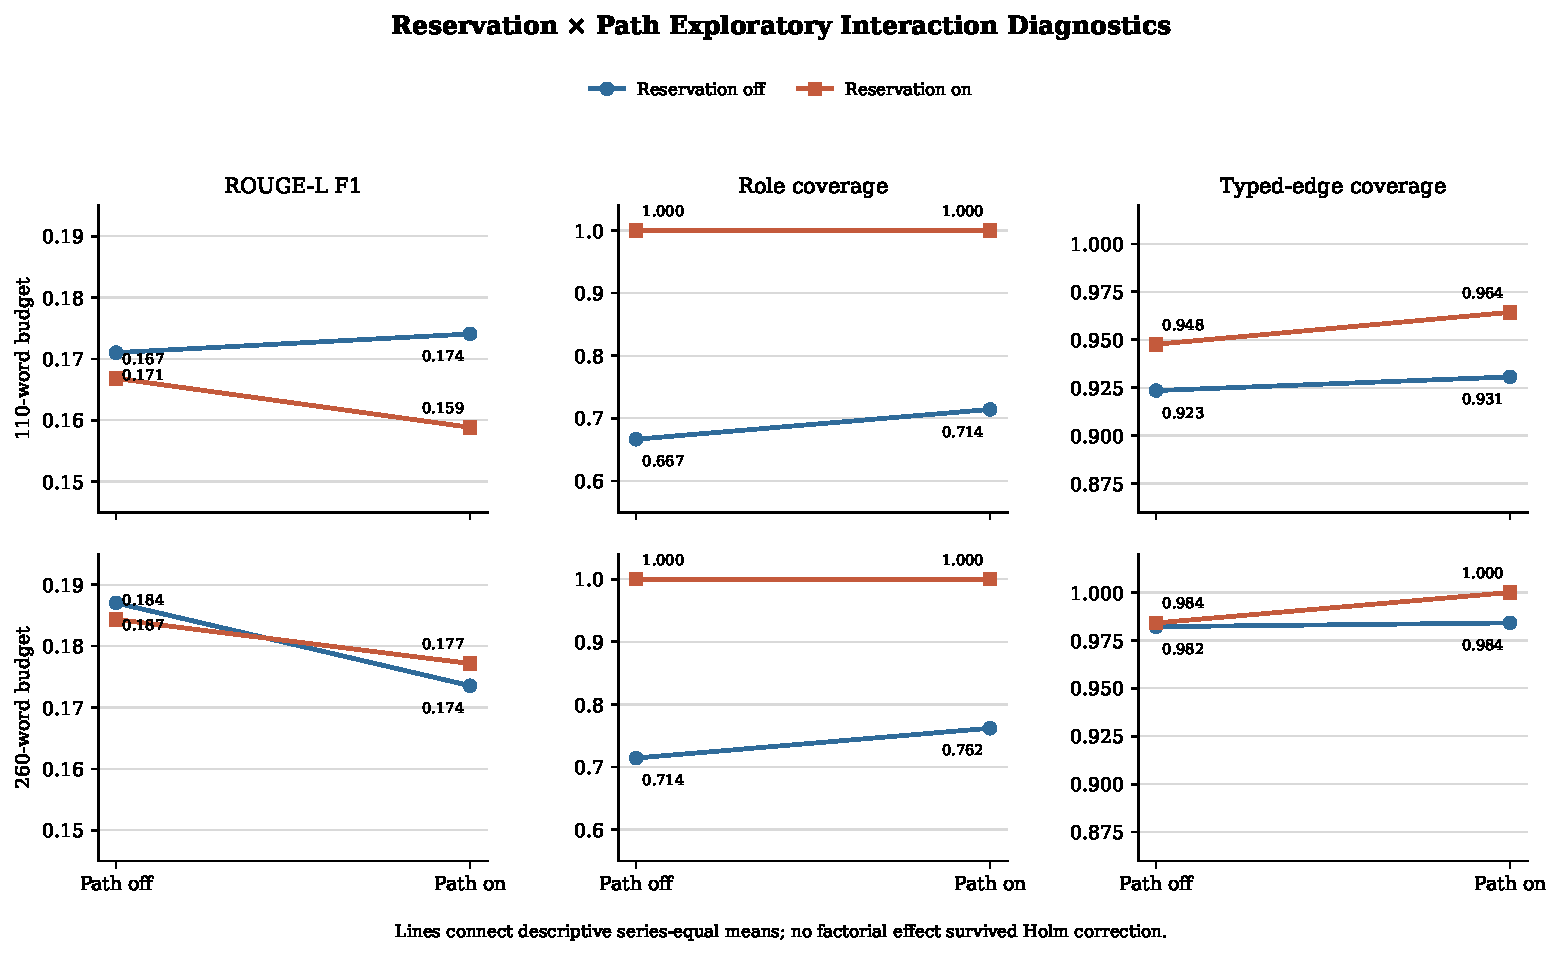
\includegraphics[width=\textwidth]{figures/figS4_reservation_path_interaction.pdf}
\end{center}

Lines compare reservation off/on while the horizontal axis switches the normalized path term. The rows show 110- and 260-word budgets; columns show ROUGE-L, formal role coverage, and formal typed-edge coverage. The budget-dependent ROUGE-L patterns do not establish a stable interaction after family-wise correction.

% ==== BEGIN ADDENDA V2 TABLES (generated) ====


\section*{Table S14. Reservation--Path Factorial Main Effects and Interaction}

Exact values behind Figure~S4, recomputed from the exploratory seven-series factorial (\nolinkurl{factorial_interactions.json}). The family was fixed for the v3 diagnostic run but not before source access, so every entry stays exploratory. Intervals are 95\% series-cluster bootstrap intervals; the exact column is the series sign-flip value and the final column its Holm adjustment inside the six-contrast family. Mean $\Delta$ is in ROUGE-L F1.

\begin{center}
\small
\resizebox{\textwidth}{!}{%
\begin{tabular}{llrrrrrr}
\toprule
Budget & Factor & Mean $\Delta$ & 95\% CI low & 95\% CI high & Paired SMD & Exact $p$ & Holm $p$\\
\midrule
110 & path channel (paths off vs on) & -0.0025 & -0.0179 & +0.0133 & -0.109 & 0.7969 & 1.0000\\
110 & role-group reservation (on vs off) & -0.0097 & -0.0175 & -0.0024 & -0.882 & 0.0469 & 0.2344\\
110 & reservation x path interaction & -0.0110 & -0.0317 & +0.0026 & -0.413 & 0.3438 & 1.0000\\
260 & path channel (paths off vs on) & -0.0103 & -0.0187 & -0.0037 & -0.930 & 0.0312 & 0.1875\\
260 & role-group reservation (on vs off) & +0.0005 & -0.0039 & +0.0053 & +0.068 & 0.8750 & 1.0000\\
260 & reservation x path interaction & +0.0063 & -0.0022 & +0.0160 & +0.478 & 0.2500 & 1.0000\\
\bottomrule
\end{tabular}}
\end{center}

Per-series deltas for the same six contrasts are supplied as \nolinkurl{q5\_reservation\_path\_series\_deltas.csv}. Neither main effect survives family-wise correction at either budget.


\section*{Table S15. External Prospective Corpus Stratified by Publisher Family}

Paired ROUGE-L F1 differences inside each publisher family of the frozen 24-report external corpus. Families are reported separately and are never pooled into a single accuracy; family sizes are 2--9, so every entry is descriptive and no test is applied. Candidate units and reference words are given as the observed range inside the family.

\begin{center}
\small
\resizebox{\textwidth}{!}{%
\begin{tabular}{llrrrrrrr}
\toprule
Family & Budget & Contrast & Reports & Candidates & Reference words & Mean $\Delta$ & neg/pos/tie\\
\midrule
ENTSO-E frequency-deviation reports & word:110 & AB2 - AB0 & 2 & 271--336 & 401--800 & -0.0834 & 2/0/0\\
ENTSO-E frequency-deviation reports & word:110 & Full - no\_path & 2 & 271--336 & 401--800 & +0.0085 & 0/2/0\\
ENTSO-E frequency-deviation reports & word:110 & TextRank - no\_path & 2 & 271--336 & 401--800 & -0.0105 & 1/1/0\\
ENTSO-E frequency-deviation reports & word:260 & AB2 - AB0 & 2 & 271--336 & 401--800 & -0.0235 & 1/1/0\\
ENTSO-E frequency-deviation reports & word:260 & Full - no\_path & 2 & 271--336 & 401--800 & -0.0799 & 2/0/0\\
ENTSO-E frequency-deviation reports & word:260 & TextRank - no\_path & 2 & 271--336 & 401--800 & -0.0893 & 1/1/0\\
ENTSO-E grid incidents & word:110 & AB2 - AB0 & 7 & 589--2000 & 1190--10935 & -0.0026 & 5/2/0\\
ENTSO-E grid incidents & word:110 & Full - no\_path & 7 & 589--2000 & 1190--10935 & -0.0010 & 2/3/2\\
ENTSO-E grid incidents & word:110 & TextRank - no\_path & 7 & 589--2000 & 1190--10935 & +0.0205 & 0/7/0\\
ENTSO-E grid incidents & word:260 & AB2 - AB0 & 7 & 589--2000 & 1190--10935 & +0.0198 & 2/5/0\\
ENTSO-E grid incidents & word:260 & Full - no\_path & 7 & 589--2000 & 1190--10935 & -0.0028 & 5/0/2\\
ENTSO-E grid incidents & word:260 & TextRank - no\_path & 7 & 589--2000 & 1190--10935 & +0.0175 & 1/6/0\\
ENTSO-E market-coupling incidents & word:110 & AB2 - AB0 & 9 & 21--84 & 108--779 & -0.0652 & 7/1/1\\
ENTSO-E market-coupling incidents & word:110 & Full - no\_path & 9 & 21--84 & 108--779 & -0.0012 & 2/0/7\\
ENTSO-E market-coupling incidents & word:110 & TextRank - no\_path & 9 & 21--84 & 108--779 & +0.0523 & 3/6/0\\
ENTSO-E market-coupling incidents & word:260 & AB2 - AB0 & 9 & 21--84 & 108--779 & -0.0614 & 5/3/1\\
ENTSO-E market-coupling incidents & word:260 & Full - no\_path & 9 & 21--84 & 108--779 & +0.0036 & 1/1/7\\
ENTSO-E market-coupling incidents & word:260 & TextRank - no\_path & 9 & 21--84 & 108--779 & +0.0604 & 3/6/0\\
NERC event reports & word:110 & AB2 - AB0 & 6 & 37--334 & 102--1431 & -0.0118 & 4/1/1\\
NERC event reports & word:110 & Full - no\_path & 6 & 37--334 & 102--1431 & -0.0060 & 2/0/4\\
NERC event reports & word:110 & TextRank - no\_path & 6 & 37--334 & 102--1431 & -0.0082 & 3/3/0\\
NERC event reports & word:260 & AB2 - AB0 & 6 & 37--334 & 102--1431 & +0.0058 & 3/3/0\\
NERC event reports & word:260 & Full - no\_path & 6 & 37--334 & 102--1431 & -0.0031 & 2/0/4\\
NERC event reports & word:260 & TextRank - no\_path & 6 & 37--334 & 102--1431 & +0.0073 & 2/4/0\\
\bottomrule
\end{tabular}}
\end{center}

The 260-word path-layer difference observed on the pooled corpus is carried by the two frequency-deviation reports; the grid-incident, market-coupling and NERC families sit close to zero. Per-condition family means are supplied as \nolinkurl{q9\_external\_family\_condition\_means.csv}.


\section*{Table S16. Per-Report Cost Against Candidate-Set Size, and Role/Edge Coverage}

Measured cost and coverage for the seven post-access external series. Candidate counts come from the private derived corpus and are reported as counts only; times are selection and scoring seconds averaged over the thirteen conditions at that budget, excluding the separately loaded embedding model. Role and typed-edge coverage are formal channel coverage, not accuracy against human judgement.

\begin{center}
\small
\resizebox{\textwidth}{!}{%
\begin{tabular}{lrrrrrr}
\toprule
Series & Candidates & Budget & Selection (s) & Peak MB & Role coverage & Typed-edge coverage\\
\midrule
series\_entsoe\_czech\_2025 & 695 & 110 & 0.082 & 1.24 & 0.846 & 0.923\\
series\_entsoe\_czech\_2025 & 695 & 260 & 0.170 & 1.43 & 0.872 & 0.978\\
series\_entsoe\_mepso\_2025 & 734 & 110 & 0.101 & 1.29 & 0.821 & 1.000\\
series\_entsoe\_mepso\_2025 & 734 & 260 & 0.203 & 1.67 & 0.872 & 0.985\\
series\_entsoe\_see\_2024 & 1408 & 110 & 0.120 & 2.47 & 0.872 & 1.000\\
series\_entsoe\_see\_2024 & 1408 & 260 & 0.263 & 2.94 & 0.872 & 1.000\\
series\_nerc\_gmd\_2024 & 200 & 110 & 0.054 & 0.40 & 0.897 & 0.936\\
series\_nerc\_gmd\_2024 & 200 & 260 & 0.087 & 0.46 & 0.949 & 0.947\\
series\_nerc\_large\_load\_loss & 58 & 110 & 0.042 & 0.23 & 0.846 & 0.931\\
series\_nerc\_large\_load\_loss & 58 & 260 & 0.064 & 0.49 & 0.872 & 0.949\\
series\_nerc\_low\_wind & 153 & 110 & 0.039 & 0.25 & 0.923 & 0.866\\
series\_nerc\_low\_wind & 153 & 260 & 0.090 & 0.44 & 0.923 & 0.922\\
series\_transpower\_tower\_130 & 830 & 110 & 0.108 & 1.60 & 0.821 & 0.729\\
series\_transpower\_tower\_130 & 830 & 260 & 0.237 & 1.86 & 0.897 & 0.814\\
\bottomrule
\end{tabular}}
\end{center}

Per-condition values, including redundancy and budget utilization, are supplied as \nolinkurl{q4\_role\_edge\_coverage\_per\_condition.csv}; the four-condition cost detail is in \nolinkurl{q3\_report\_cost\_vs\_candidates.csv}.


\section*{Table S17. One-Sided Bounds on the Frozen External Layer Contrasts}

Post hoc bounds computed on the same frozen 24-report record as Table~S10 and the arm-level experiment. The upper limit is the one-sided 95\% bootstrap percentile of the paired mean difference (200\,000 resamples, seed 20260926), i.e. the largest gain still compatible with the data. The leave-one-out columns report the span of the mean and the worst-case upper limit when any single report is removed. Bounds are post hoc and are not pre-registered confirmatory tests.

\begin{center}
\small
\resizebox{\textwidth}{!}{%
\begin{tabular}{llrrrrrr}
\toprule
Contrast & Budget & Reports & Mean $\Delta$ & neg/pos/tie & Upper limit (95\%) & LOO mean range & LOO worst limit\\
\midrule
path layer (Full $-$ no-path) & unit:10 & 24 & +0.0010 & 8/6/10 & +0.0038 & [+0.0001, +0.0016] & +0.0043\\
path layer (Full $-$ no-path) & unit:5 & 24 & -0.0005 & 5/4/15 & +0.0047 & [-0.0026, +0.0012] & +0.0059\\
path layer (Full $-$ no-path) & word:110 & 24 & -0.0015 & 6/5/13 & +0.0006 & [-0.0020, -0.0004] & +0.0012\\
path layer (Full $-$ no-path) & word:260 & 24 & -0.0069 & 10/1/13 & +0.0021 & [-0.0094, -0.0006] & +0.0038\\
role layer (AB-2 $-$ AB-0) & unit:10 & 24 & +0.0108 & 9/15/0 & +0.0228 & [+0.0074, +0.0146] & +0.0255\\
role layer (AB-2 $-$ AB-0) & unit:5 & 24 & +0.0063 & 10/14/0 & +0.0180 & [+0.0036, +0.0126] & +0.0209\\
role layer (AB-2 $-$ AB-0) & word:110 & 24 & -0.0351 & 18/4/2 & -0.0166 & [-0.0385, -0.0287] & -0.0125\\
role layer (AB-2 $-$ AB-0) & word:260 & 24 & -0.0178 & 11/12/1 & +0.0033 & [-0.0207, -0.0074] & +0.0077\\
TextRank baseline & word:110 & 24 & +0.0227 & 7/17/0 & +0.0442 & [+0.0140, +0.0280] & +0.0492\\
TextRank baseline & word:260 & 24 & +0.0221 & 7/17/0 & +0.0440 & [+0.0154, +0.0316] & +0.0503\\
Lead baseline & word:110 & 24 & +0.0104 & 9/15/0 & +0.0276 & [+0.0038, +0.0133] & +0.0306\\
Lead baseline & word:260 & 24 & +0.0172 & 10/14/0 & +0.0372 & [+0.0092, +0.0209] & +0.0407\\
\bottomrule
\end{tabular}}
\end{center}

The path-layer upper limit stays at or below $+0.0047$ in every budget and at or below $+0.0059$ under leave-one-out, so a path-channel gain larger than $+0.005$ ROUGE-L is excluded on this corpus even though the mean-based test is not significant. The role-layer upper limit is positive under equal-unit budgets and negative at 110 words, which is the budget dependence reported in the main text.

\section*{Figure S5. Budget-Efficiency Curves on the Frozen External Corpus}

\begin{center}
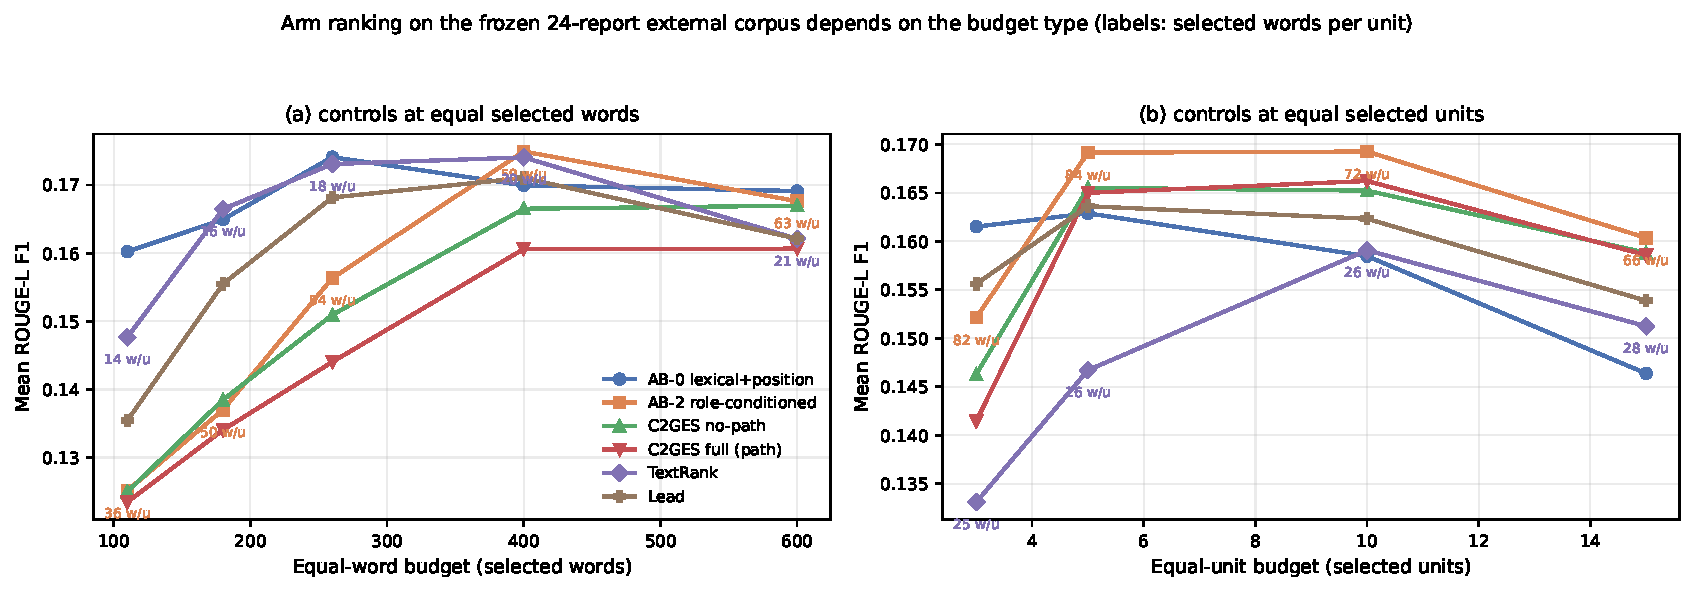
\includegraphics[width=\textwidth]{figures/figS5_budget_efficiency_curve.pdf}
\end{center}

Panel (a) holds the selected-word budget fixed (110--600 words) and panel (b) the selected-unit budget (3--15 units); labels give the realised selected words per unit. The ordering of the arms is a property of the budget type: TextRank and Lead lead at mid-range word budgets, whereas the role-conditioned arms lead under equal-unit budgets while packing roughly 1.5 times as many words per selected unit as the lexical-and-position baseline and about three times as many as TextRank. Source values are supplied as \nolinkurl{figS5_source.csv} and the full arm record as \nolinkurl{external\_arms\_curve\_v4.json}.


\section*{Table S18. Out-of-Domain Transfer Check on GovReport}

The frozen arm set applied without tuning to 100 length-stratified documents from the GovReport test split (CRS and GAO reports with human-written summaries, CC BY 4.0; drawn with seed 20260926 from 973 test rows). This is a robustness transfer layer, not domain evidence: the role cue lexicon is power-domain specific (mean formal role coverage 0.246, minimum 0.016) and the references are abstractive. Intervals and limits are computed as in Table~S17 (200\,000 bootstrap samples).

\begin{center}
\small
\resizebox{\textwidth}{!}{%
\begin{tabular}{llrrrrrr}
\toprule
Contrast & Budget & Reports & Mean $\Delta$ & neg/pos/tie & Upper limit (95\%) & LOO mean range & LOO worst limit\\
\midrule
path layer (Full $-$ no-path) & word:110 & 100 & -0.0031 & 24/15/61 & -0.0011 & [-0.0033, -0.0019] & -0.0006\\
path layer (Full $-$ no-path) & word:260 & 100 & -0.0026 & 37/25/38 & -0.0007 & [-0.0031, -0.0022] & -0.0004\\
path layer (Full $-$ no-path) & unit:5 & 100 & -0.0052 & 39/13/48 & -0.0030 & [-0.0055, -0.0044] & -0.0025\\
path layer (Full $-$ no-path) & unit:10 & 100 & -0.0028 & 30/21/49 & -0.0010 & [-0.0030, -0.0024] & -0.0007\\
role layer (AB-2 $-$ AB-0) & word:110 & 100 & -0.0212 & 81/17/2 & -0.0161 & [-0.0220, -0.0200] & -0.0149\\
role layer (AB-2 $-$ AB-0) & word:260 & 100 & -0.0204 & 77/22/1 & -0.0143 & [-0.0218, -0.0195] & -0.0135\\
role layer (AB-2 $-$ AB-0) & unit:5 & 100 & -0.0007 & 52/48/0 & +0.0062 & [-0.0028, +0.0006] & +0.0072\\
role layer (AB-2 $-$ AB-0) & unit:10 & 100 & -0.0098 & 71/29/0 & -0.0038 & [-0.0111, -0.0087] & -0.0030\\
TextRank $-$ no-path & word:110 & 100 & +0.0215 & 15/84/1 & +0.0264 & [+0.0209, +0.0230] & +0.0274\\
TextRank $-$ no-path & word:260 & 100 & +0.0273 & 14/86/0 & +0.0332 & [+0.0264, +0.0287] & +0.0342\\
TextRank $-$ no-path & unit:5 & 100 & +0.0005 & 43/57/0 & +0.0072 & [-0.0003, +0.0029] & +0.0085\\
TextRank $-$ no-path & unit:10 & 100 & +0.0119 & 33/67/0 & +0.0182 & [+0.0109, +0.0138] & +0.0194\\
Lead $-$ no-path & word:110 & 100 & +0.0034 & 57/42/1 & +0.0123 & [+0.0007, +0.0043] & +0.0132\\
Lead $-$ no-path & word:260 & 100 & +0.0044 & 62/38/0 & +0.0170 & [-0.0005, +0.0056] & +0.0182\\
Lead $-$ no-path & unit:5 & 100 & -0.0250 & 81/19/0 & -0.0113 & [-0.0308, -0.0238] & -0.0101\\
Lead $-$ no-path & unit:10 & 100 & -0.0166 & 74/26/0 & -0.0038 & [-0.0203, -0.0153] & -0.0024\\
\bottomrule
\end{tabular}}
\end{center}

Every path-layer upper limit is below zero, so a positive path-channel effect is excluded on this corpus at all four budgets, and the role-conditioned arms are significantly worse than their lexical baseline at both word budgets. Per-document records are supplied as \nolinkurl{govreport\_transfer\_v1.json}.

\textbf{Sensitivity: the frozen strata fully sampled (970 of 973 test rows).} The same frozen protocol run over every document of the five strata, as a sensitivity rather than a new pre-registered test. Holm values are those of the full arm-by-budget family (twelve contrasts).

\begin{center}
\small
\resizebox{\textwidth}{!}{%
\begin{tabular}{llrrrr}
\toprule
Contrast & Budget & Reports & Mean $\Delta$ & neg/pos/tie & Upper limit (95\%)\\
\midrule
path layer (Full $-$ no-path) & word:110 & 970 & -0.0021 & 233/156/581 & -0.0013\\
path layer (Full $-$ no-path) & word:260 & 970 & -0.0017 & 330/224/416 & -0.0008\\
path layer (Full $-$ no-path) & unit:5 & 970 & -0.0032 & 316/166/488 & -0.0024\\
path layer (Full $-$ no-path) & unit:10 & 970 & -0.0020 & 306/197/467 & -0.0013\\
role layer (AB-2 $-$ AB-0) & word:110 & 970 & -0.0193 & 722/233/15 & -0.0175\\
role layer (AB-2 $-$ AB-0) & word:260 & 970 & -0.0220 & 725/241/4 & -0.0199\\
role layer (AB-2 $-$ AB-0) & unit:5 & 970 & -0.0030 & 508/460/2 & -0.0009\\
role layer (AB-2 $-$ AB-0) & unit:10 & 970 & -0.0134 & 632/337/1 & -0.0112\\
\bottomrule
\end{tabular}}
\end{center}

Every path-layer upper limit remains below zero at $n=970$ (worst case $-0.0008$), and the path contrasts are family-corrected significant at all four budgets (Holm $0.0002$--$0.0040$); the role layer is negative at every budget as well. Pairwise records are supplied as \nolinkurl{govreport\_transfer\_full970\_pairs.csv}.

\textbf{Energy-topic subset of the same split (160 documents).} Selecting reports whose body matches at least three entries of a frozen keyword list (energy, grid, transmission, power plant, electricity, renewable, nuclear, and so on; the rule was fixed before the subset was formed) gives a topic stratum that is closer to the paper's domain than the full split. The path-layer differences at the four budgets are -0.0009 / -0.0016 / -0.0018 / -0.0025, every positive share of discordant documents is at or below 41\%, and the worst one-sided 95\% upper limit is $+0.0008$, so the $+0.005$ margin still holds; the ten-unit contrast is family-corrected significant (Holm $0.0174$) while the word-budget contrasts are not. Records: \nolinkurl{govreport\_energy160\_pairs.csv}.


\section*{Table S19. Reference-Type Sensitivity with Human-Written Highlights}

The frozen arm set applied to 400 length-stratified CNN/DailyMail test articles whose reference is the human-written highlight bullet points rather than an abstractive summary. This is a reference-type sensitivity, not domain evidence: the corpus is news, the articles are short (median 23 candidate units), and the power-domain cue lexicon barely applies (mean formal role coverage 0.116). The point of the layer is that the path channel leaves the selection untouched in almost every document, so a null cannot be an artefact of comparing extracts with rewritten text.

\begin{center}
\small
\resizebox{\textwidth}{!}{%
\begin{tabular}{llrrrr}
\toprule
Contrast & Budget & Articles & Mean $\Delta$ & neg/pos/tie & Upper limit (95\%)\\
\midrule
path layer (Full $-$ no-path) & word:110 & 400 & +0.0005 & 14/10/376 & +0.0016\\
path layer (Full $-$ no-path) & word:260 & 400 & -0.0003 & 18/14/368 & +0.0002\\
path layer (Full $-$ no-path) & unit:5 & 400 & -0.0000 & 4/4/392 & +0.0002\\
path layer (Full $-$ no-path) & unit:10 & 400 & +0.0000 & 1/4/395 & +0.0000\\
role layer (AB-2 $-$ AB-0) & word:110 & 400 & -0.0092 & 187/135/78 & -0.0055\\
role layer (AB-2 $-$ AB-0) & word:260 & 400 & -0.0018 & 134/119/147 & -0.0005\\
role layer (AB-2 $-$ AB-0) & unit:5 & 400 & -0.0065 & 180/131/89 & -0.0034\\
role layer (AB-2 $-$ AB-0) & unit:10 & 400 & -0.0013 & 125/130/145 & +0.0003\\
\bottomrule
\end{tabular}}
\end{center}

The path-layer difference is zero to the fourth decimal at three of the four budgets, with 92--99\% of articles exactly tied, and every one-sided upper limit is at most $+0.0016$ --- far inside the $+0.005$ margin. Under this reference the term is inert rather than harmful, and the position baseline dominates (Lead's advantage is family-corrected significant at all four budgets). Per-document pairs are supplied as \nolinkurl{reference\_type\_400\_pairs.csv}.


\section*{Table S20. Frozen Parent--Held-Out Synthetic Stress Fixtures}

Sixteen fictional reports in eight series generated under the frozen protocol \nolinkurl{PROTOCOL\_synthetic\_c2ges\_gendata\_v1.md} (sha256 prefix daf7c969, thresholds unchanged after freezing) and shipped with the run manifests, gate ledgers, dataset card and the component-factorial records. The parent and held-out sets use disjoint themes, and the two generator families are swapped between them. All nineteen deterministic gates pass in both sets; the fixtures are software and endpoint stress material and never enter the E1/E2/E3 evidence chain.

\begin{center}
\small
\resizebox{\textwidth}{!}{%
\begin{tabular}{llrrllrr}
\toprule
Set & Method & 110 words & 260 words & Set & Method & 110 words & 260 words\\
\midrule
Parent & Full \cges{} & 0.1302 & 0.1184 & Held-out & Full \cges{} & 0.1168 & 0.1082\\
Parent & No-path \cges{} & 0.1199 & 0.1086 & Held-out & No-path \cges{} & 0.1171 & 0.1039\\
Parent & G-T (typed, no path) & 0.1199 & 0.1086 & Held-out & G-T (typed, no path) & 0.1171 & 0.1039\\
Parent & G-U (untyped, no path) & 0.0887 & 0.0981 & Held-out & G-U (untyped, no path) & 0.0826 & 0.0910\\
\bottomrule
\end{tabular}}
\end{center}

Full--no-path macro-mean differences (110/260 words) match the table: parent +0.0103 / +0.0098; held-out -0.0003 / +0.0043. Series-equal Full--no-path (110/260 words): parent Full$-$no-path +0.0147 / +0.0178 (Holm 0.75 / 0.75); held-out Full$-$no-path -0.0007 / +0.0032 (Holm 1.00 / 1.00). Typed-minus-untyped graph: parent G-T$-$G-U +0.0312 / +0.0104 (Holm 0.25 / 0.25); held-out G-T$-$G-U +0.0344 / +0.0129 (Holm 0.25 / 0.25). Reservation main effect: parent reservation +0.0089 / -0.0098 (Holm 1.00 / 1.00); held-out reservation +0.0040 / +0.0111 (Holm 1.00 / 1.00). No corrected path contrast is nonzero in either set.

\begin{center}
\small
\resizebox{\textwidth}{!}{%
\begin{tabular}{lllll}
\toprule
Gate & Frozen rule (abridged) & Parent measured & Held-out measured & Pass\\
\midrule
S1 & 4 series x 2 reports each & 8/8 & 8/8 & 19/19\\
S2 & reference equals the concatenation of reference\_unit\_ids & 8/8 & 8/8 & 19/19\\
S3 & causal DAG acyclic & 8/8 & 8/8 & 19/19\\
S4 & semantic core 18--26 sentences; 10--28 words & 8/8 & 8/8 & 19/19\\
S5 & five roles x 2--6 each, non-uniform; one priority=2 per role & 8/8 & 8/8 & 19/19\\
S6 & every report covers all five roles & 8/8 & 8/8 & 19/19\\
S7 & Synthetic facility prefix; forbidden tokens zero & 8/8 & 8/8 & 19/19\\
S8 & 24--36 distinct distractors; 10--24 words & 8/8 & 8/8 & 19/19\\
D1 & candidate-count W1 <= 0.75 & 0.208 & 0.208 & 19/19\\
D2 & page-count W1 <= 0.75 & 0.131 & 0.131 & 19/19\\
D3 & layout-share max abs(delta) <= 0.03 & 0.000 & 0.000 & 19/19\\
D4 & exact duplicate rate <= 0.20 & 0.000 & 0.000 & 19/19\\
D5 & unit-length W1 <= 0.25 & 0.189 & 0.174 & 19/19\\
D7 & core-sentence first-quartile share <= 0.25 & 0.000--0.250 & 0.000--0.238 & 19/19\\
D8 & max Jaccard vs real corpus <= 0.15; hit share <= 2\% & 0.120 / 0.000 & 0.062 / 0.000 & 19/19\\
D9 & distractor families >= 6; single family <= 40\% & 150--675 / 0.011 & 150--675 / 0.028 & 19/19\\
E1b & within-set per-report AUROC >= 0.80 & 0.894--0.970 & 0.875--0.945 & 19/19\\
E2 & distinct-2 >= 0.526 & 0.452--0.656 & 0.535--0.656 & 19/19\\
E3 & vocabulary overlap >= 0.55 & 0.675 & 0.627 & 19/19\\
\bottomrule
\end{tabular}}
\end{center}

The leakage gate D8 keeps every unit's maximum Jaccard overlap with the real corpus at or below 0.12 (parent) / 0.06 (held-out) against a frozen 0.15 bound; E1b is the within-set per-report document-identity AUROC (frozen floor 0.80), E2 is distinct-2 and E3 is vocabulary overlap with the development lexicon. AUROC(synthetic-vs-real) is reported but descriptive only: it measures document identity, not realism. The fixture is a synthetic assembly with visible seams at distractor joints, an easily separable document identity, and only eight reports per set, so it supports software and mechanism diagnosis but not statistical inference; the parent line saw generator-side tuning on intermediate gate results (thresholds unchanged) and the held-out line is the independent check (README and dataset card shipped beside the records). Records: \nolinkurl{synthetic\_stress\_v1/run\_20260927\_gendata\_parent\_v3r1/} and \nolinkurl{synthetic\_stress\_v1/run\_20260927\_gendata\_heldout\_v2r3/}.


% ==== END ADDENDA V2 TABLES ====

\section*{Exploratory Development-Only Calibration}

The complete chronology, configuration space, leave-one-report-out results, and machine-readable records are described in \nolinkurl{03_Reproducibility/Data/POST_UNBLINDING_DEV_CALIBRATION_SUPPLEMENT.md}. A zero path-deletion weight was selected in all 12 development folds; the analysis was not applied to the retained 15-report test set.

A separate equal-budget exercise is documented in \nolinkurl{03_Reproducibility/Data/dev_balanced_tuning/}. Semantic-MMR, TextRank, and normalized-path \cges{} each received nine configurations and the same ordered development objective over both extraction budgets. The selected values were 0.9, 0.65, and 0.0, respectively. The decision record states \nolinkurl{test_input_accessed=false}; these configurations are authorized only for a future preregistered external-series comparison and do not alter the retained-test results.

\end{document}
